\documentclass[9pt]{beamer}

\usepackage[utf8]{inputenc}

\RequirePackage{tikz}
\usetikzlibrary{arrows}
\graphicspath{{../images/theme/}}

\usetheme{default}
\useinnertheme[shadow]{rounded}

%\useoutertheme[left,hideothersubsections]{IGNsidebar}
\usepackage[left,hideothersubsections]{./includes/beamerouterthemeIGNsidebar}




%/usr/share/texmf/tex/latex/beamer/themes/font/beamerfontthemedefault.sty
%/usr/share/texmf/tex/latex/beamer/themes/font/beamerfontthemeprofessionalfonts.sty
%/usr/share/texmf/tex/latex/beamer/themes/font/beamerfontthemeserif.sty
%/usr/share/texmf/tex/latex/beamer/themes/font/beamerfontthemestructurebold.sty
%/usr/share/texmf/tex/latex/beamer/themes/font/beamerfontthemestructureitalicserif.sty
%/usr/share/texmf/tex/latex/beamer/themes/font/beamerfontthemestructuresmallcapsserif.sty
\usefonttheme{structurebold}

\RequirePackage{tikz}

\definecolor{IGNVert}{RGB}{148, 192,  22}
\definecolor{IGNGris}{RGB}{112, 119, 122}

\definecolor{IGNRouge}{RGB}{255, 100, 100}

%PUCES
\setbeamercolor{item projected}{bg=IGNGris!70}

%%%%%%%%%%%%%%%%%%%%%%%%%%%%%%%%%%%%%%%%%%%%%%%%%%% COLOR
\setbeamercolor*{normal text}{fg=IGNGris}

\setbeamercolor{title}{fg=IGNGris}
\setbeamercolor{subtitle}{fg=IGNVert}
\setbeamercolor{item}{fg=IGNVert} 

\setbeamercolor{caption name}{ fg=IGNGris}

\setbeamercolor{author in head/foot}{ fg=IGNGris}
\setbeamercolor{institute in head/foot}{fg=IGNGris}
\setbeamercolor{title in head/foot}{ fg=IGNGris}
\setbeamercolor{date in head/foot}{ fg=IGNGris}
\setbeamercolor{page in head/foot}{ fg=IGNGris}
\setbeamercolor{section in toc}{ fg=IGNGris}
\setbeamercolor{subsection in toc}{ fg=IGNGris}

\setbeamercolor*{block title alerted}{bg=IGNRouge!70}
\setbeamercolor*{block body alerted}{bg=IGNRouge!20}

\setbeamercolor*{block title example}{bg=IGNVert!70}
\setbeamercolor*{block body example}{bg=IGNVert!20}

\setbeamercolor*{block title}{bg=IGNGris!50}
\setbeamercolor*{block body}{bg=IGNGris!20}

%%%%%%%%%%%%%%%%%%%%%%%%%%%%%%%%%%%%%%%%%%%%%%%%%%% NAVIGATION SYMBOLS
\setbeamertemplate{navigation symbols}{} 
%%%%%%%%%%%%%%%%%%%%%%%%%%%%%%%%%%%%%%%%%%%%%%%%%%% SIDE BAR
\setbeamersize{sidebar width left=1.2cm}
\setbeamercolor{section in sidebar}{fg=IGNGris}
\setbeamercolor{subsection in sidebar}{fg=IGNGris}

\setbeamercolor{section in sidebar shaded}{fg=IGNVert}
\setbeamercolor{subsection in sidebar shaded}{fg=IGNVert}


\defbeamertemplate*{sidebar}{SSB}{}

%%%%%%%%%%%%%%%%%%%%%%%%%%%%%%%%%%%%%%%%%%%%%%%%%%% HEAD LINE
\defbeamertemplate*{frametitle}{}{
  \begin{tikzpicture}[scale=0.503]
  \filldraw[color=white] (0,0) rectangle(0.1,0.54);
  \end{tikzpicture}
  
    \textcolor{IGNGris}{ \textbf{\insertframetitle}}
  
\begin{tikzpicture}
  \draw[very thick,color=IGNVert] (0,1)--(\paperwidth- 2.24,1);
  \end{tikzpicture} 
}
%%%%%%%%%%%%%%%%%%%%%%%%%%%%%%%%%%%%%%%%%%%%%%%%%%% HEAD LINE
%\defbeamertemplate*{headline}{AH}{
%}

\defbeamertemplate*{headline}{}{}
%%%%%%%%%%%%%%%%%%%%%%%%%%%%%%%%%%%%%%%%%%%%%%%%%%% BACKGROUND

%%%%%%%%%%%%%%%%%%%%%%%%%%%%%%%%%%%%%%%%%%%%%%%%%%% FOOT LINE
\defbeamertemplate*{footline}{}
{
\leavevmode%
  \begin{tikzpicture}
  \draw (0,0) node  {};
  \draw (0.5,0) node[right]  { \textcolor{IGNGris}{\insertshorttitle}};
  \draw (5,0) node[right]  { \textcolor{IGNVert}{$\blacksquare$} \textcolor{IGNGris}{\insertshortdate{} } };
  \draw (7.5,0) node  { \textcolor{IGNVert}{$\blacksquare$} \textcolor{IGNGris}{\insertframenumber{} / \inserttotalframenumber\hspace*{2ex} }};
  \draw (9.75,0) node  { \textcolor{IGNGris}{ \insertinstitute }};
  \draw (12,0) node[right] { 
\includegraphics[height=0.25cm]{LOGO_IGN_p.png} };
  \end{tikzpicture} 

}%


%%%%%%%%%%%%%%%%%%%%%%%%%%%%%%%%%%%%%%%%%%%%%%%%%%% AT BEGIN SECTION


\AtBeginSection[]
{ 
\setbeamercolor{section in sidebar}{fg=white }
\setbeamercolor{subsection in sidebar}{fg=white }

\setbeamercolor{section in sidebar shaded}{fg=white }
\setbeamercolor{subsection in sidebar shaded}{fg=white }



\begin{frame}{
  
\begin{tikzpicture}[scale=0.503]
  \draw[color=IGNGris,fill=IGNGris]  (0,0) rectangle (23,9);
  \draw (1,1) node [right,text width=10cm,text justified]  {  \textcolor{white}{\insertsection}};
  \end{tikzpicture}
}
\end{frame} 


\setbeamercolor{section in sidebar}{fg=IGNGris}
\setbeamercolor{subsection in sidebar}{fg=IGNGris}

\setbeamercolor{section in sidebar shaded}{fg=IGNVert}
\setbeamercolor{subsection in sidebar shaded}{fg=IGNVert}

\addtocounter{framenumber}{-1}

}


\usepackage[acronym]{glossaries}
\newacronym{acr::sample}{Accro}{Acronym}


\usepackage{amssymb}
\usepackage{amsmath}

\usepackage{mathtools}
\DeclarePairedDelimiter\ceil{\lceil}{\rceil}
\DeclarePairedDelimiter\norm{\vert\vert}{\vert\vert}
\DeclarePairedDelimiter\abs{\vert}{\vert}

\usepackage{hyperref}

\usepackage{color}


\title{Title}
\subtitle{SubTitle:}
\author{Author McAuthor}
\institute{IGN | K316}
\date{\today}


\AtBeginSubsection[]
{
	\begin{frame}<beamer>
		\frametitle{Presentation Layout}
		\tableofcontents[
		currentsection,
		sectionstyle=show/shaded,
		subsectionstyle=show/shaded/hide
		]
	\end{frame}
}

\AtBeginSection[]
{
	\begin{frame}<beamer>
		\frametitle{Presentation Layout}
		\tableofcontents[
		currentsection,
		sectionstyle=show/shaded,
		subsectionstyle=hide
		]
	\end{frame}
}

\begin{document}
	% Cover layout
	\usebackgroundtemplate{
		\begin{tikzpicture}
			\draw (0,0.5) node[right] { 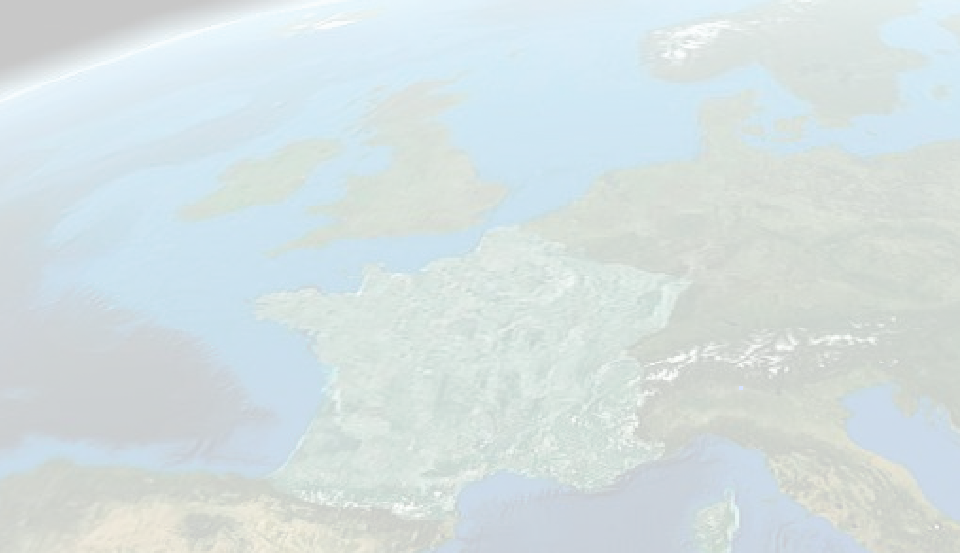
\includegraphics[width=12.5cm]{fondClair.png} };
			\draw (0,5) node[right] { 
\includegraphics[height=1.5cm]{LOGO_IGN.png} };
			\draw (1.5,4.95) node[right] { 
\includegraphics[width=3cm]{fondD.jpg} };
		\end{tikzpicture}   
	}
	
	\begin{frame}[plain,c]
		\begin{columns}
			\begin{column}{8cm}
				\begin{center}
					\vspace{2cm}
					\titlepage
				\end{center}
			\end{column}
			\begin{column}{1cm}
			\end{column}
		\end{columns}
	\end{frame}
	
	% Background layout
	\usebackgroundtemplate{
		
\begin{tikzpicture}[scale=0.503]
			\filldraw[color=IGNGris] (0,0) rectangle(2.62,0.54);
			\filldraw[color=IGNGris] (4.77,0) rectangle(2.62+4.77,0.54);
			
			\filldraw[color=IGNVert] (9.50+0.27,0) -- (9.50,0.54)-- (9.50+7.41-0.27,0.54)-- (9.50+7.41,0)--cycle;
			
			\filldraw[color=IGNGris] (19.50,0) rectangle(2.62+19.50,0.54);
			\filldraw[color=IGNGris] (23.11,0.54)--(23.11+0.54,0)--(2.3+23.11,0)--(2.3+23.11,0.54)--cycle;;
		\end{tikzpicture}   
	}
		
	% Plan layout
	\setbeamercolor{section in sidebar}{fg=white } %LIGNE NECESSAIRE POUR EFFACER LE PLAN DE LA SIDEBAR (PAS MIEUX)
	\setbeamercolor{subsection in sidebar}{fg=white }%LIGNE NECESSAIRE POUR EFFACER LE PLAN DE LA SIDEBAR (PAS MIEUX)
	\setbeamercolor{section in sidebar shaded}{fg=white }%LIGNE NECESSAIRE POUR EFFACER LE PLAN DE LA SIDEBAR (PAS MIEUX)
	\setbeamercolor{subsection in sidebar shaded}{fg=white }%LIGNE NECESSAIRE POUR EFFACER LE PLAN DE LA SIDEBAR (PAS MIEUX)
	\begin{frame}
		\tableofcontents
	\end{frame}
	\setbeamercolor{section in sidebar}{fg=IGNGris}%LIGNE NECESSAIRE POUR AFFICHER LE PLAN DE LA SIDEBAR (PAS MIEUX)
	\setbeamercolor{subsection in sidebar}{fg=IGNGris}%LIGNE NECESSAIRE POUR AFFICHER LE PLAN DE LA SIDEBAR (PAS MIEUX)
	\setbeamercolor{section in sidebar shaded}{fg=IGNVert}%LIGNE NECESSAIRE POUR AFFICHER LE PLAN DE LA SIDEBAR (PAS MIEUX)
	\setbeamercolor{subsection in sidebar shaded}{fg=IGNVert}%LIGNE NECESSAIRE POUR AFFICHER LE PLAN DE LA SIDEBAR (PAS MIEUX)



	\section*{Introduction}
	\begin{frame}{Introduction}
		\begin{itemize}
			\item[-] Say something here.
		\end{itemize}
	\end{frame}
	
		
%%%%%%%%%%%%%%%%%%%%%%%%%%%%%%%%%%%%%%%%%%%%%%%%%%%%%%%%%%%%%%%%%%%%%%%%%%%%%%%%%%%%%%%%%%%%%%%%%%%%%%%%%
%%% SECTION
%%%%%%%%%%%%%%%%%%%%%%%%%%%%%%%%%%%%%%%%%%%%%%%%%%%%%%%%%%%%%%%%%%%%%%%%%%%%%%%%%%%%%%%%%%%%%%%%%%%%%%%%%
\section[Motivation]{Motivation:}

%%%%%%%%%%%%%%%%%%%%%%%%%%%%%%%%%%%%%%%%%%%%%%%%%%%%%%%%%%%%%%%%%%%%%%%%%%%%%%%%%%%%%%%%%%%%%%%%%%%%%%%%%
%%% SOUS SECTION
%%%%%%%%%%%%%%%%%%%%%%%%%%%%%%%%%%%%%%%%%%%%%%%%%%%%%%%%%%%%%%%%%%%%%%%%%%%%%%%%%%%%%%%%%%%%%%%%%%%%%%%%%
\subsection[Dimensionality]{Curse of dimensionality:}
\begin{frame}{Curse of dimensionality:}
	Some issues to take into account:
	\begin{itemize}
		\item[-] Samples cover exponenetially less volume while dimension grows: you need at least $ \ceil*{\frac{1}{\epsilon}^d}$ points to cover uniformly a hypercube, with a side length of $1$, at distance $\epsilon$.
		\item[-] Most intuition comming from low dimensions ( $ d < 2$ ) are not always valid: 
		\begin{itemize}
			\item[-] For instance, there is more volume in the corners of a hypercube rather than the center:
			$$\frac{V(\mathbb{B}_{2}(r))}{V(\mathbb{B}_{\infty}(r))}\xrightarrow[d \to \infty]{} 0$$
			\item[-] As the dimensionality increases, the less Euclidian distances are meaningful \cite{Domingos:2012:FUT:2347736.2347755}.
		\end{itemize}
	\end{itemize}
\end{frame}


%%%%%%%%%%%%%%%%%%%%%%%%%%%%%%%%%%%%%%%%%%%%%%%%%%%%%%%%%%%%%%%%%%%%%%%%%%%%%%%%%%%%%%%%%%%%%%%%%%%%%%%%%

%%%%%%%%%%%%%%%%%%%%%%%%%%%%%%%%%%%%%%%%%%%%%%%%%%%%%%%%%%%%%%%%%%%%%%%%%%%%%%%%%%%%%%%%%%%%%%%%%%%%%%%%%
%%% SECTION
%%%%%%%%%%%%%%%%%%%%%%%%%%%%%%%%%%%%%%%%%%%%%%%%%%%%%%%%%%%%%%%%%%%%%%%%%%%%%%%%%%%%%%%%%%%%%%%%%%%%%%%%%
\section[Scattering]{Scattering Transform:}

%%%%%%%%%%%%%%%%%%%%%%%%%%%%%%%%%%%%%%%%%%%%%%%%%%%%%%%%%%%%%%%%%%%%%%%%%%%%%%%%%%%%%%%%%%%%%%%%%%%%%%%%%

%%%%%%%%%%%%%%%%%%%%%%%%%%%%%%%%%%%%%%%%%%%%%%%%%%%%%%%%%%%%%%%%%%%%%%%%%%%%%%%%%%%%%%%%%%%%%%%%%%%%%%%%%
\subsection[Properties]{Mathematical Properties:}
\begin{frame}{Mathematical Properties:}
	\begin{block}{Scattering invariance properties:}
		\begin{itemize}
			\item[(i).] Let $G$ be a group. We note the action of $g \in G $ on an image $x(u)$: $x_g(u) = x(g^{-1}.u)$. We want the representation $\Phi$ to be invariant to the action of $G$ \cite{sifre2013rotation} iif :
			\begin{equation}
				\Phi(x_g)=\Phi(x)
			\end{equation}
			\item[(ii).] We want the representation $\Phi$ to be contractive \cite{anden2014deep} in order to preserve similarity:
			\begin{equation}
				\norm*{\Phi(x)-\Phi(y)} \leq \norm*{x-y}
			\end{equation}
			\item[(iii).] We want the representation to be stable to small deformations \cite{mallat2012group}: for any diffeomorphism $\tau$ such that $ \norm*{\nabla \tau} < 1$, 
			\begin{equation}
				\norm*{\Phi(x) - \Phi(x_{\tau})} \leq C.\norm*{\nabla \tau}.\norm*{x}
			\end{equation}
		\end{itemize}
	\end{block}
\end{frame}

%%%%%%%%%%%%%%%%%%%%%%%%%%%%%%%%%%%%%%%%%%%%%%%%%%%%%%%%%%%%%%%%%%%%%%%%%%%%%%%%%%%%%%%%%%%%%%%%%%%%%%%%%
%%% SECTION
%%%%%%%%%%%%%%%%%%%%%%%%%%%%%%%%%%%%%%%%%%%%%%%%%%%%%%%%%%%%%%%%%%%%%%%%%%%%%%%%%%%%%%%%%%%%%%%%%%%%%%%%%
\section[Issues]{Practical Issues:}

%%%%%%%%%%%%%%%%%%%%%%%%%%%%%%%%%%%%%%%%%%%%%%%%%%%%%%%%%%%%%%%%%%%%%%%%%%%%%%%%%%%%%%%%%%%%%%%%%%%%%%%%%
\subsection[Numerical]{Numerical considerations:}

\begin{frame}{Numerical considerations:}
	\begin{itemize}
		\item[-] We scatter only along frequency decreasing paths $0<j_k\leq j_{k+1}<J$. Other coefficients are close to zero.
		\item[-] Most of the energy of the transform is concentrated in the first layers:
		\item[-] Implementations:
		\begin{itemize}
			\item[-] \href{https://github.com/scatnet/scatnet}{ScatNet available on GitHub} (Apache 2.0).
		\end{itemize}
	\end{itemize}
\end{frame}

\subsection[Textures]{Texture discrimination:}

\subsection[Comparison]{Comparison with :}

	
	
	\section*{References}
	\begin{frame}[allowframebreaks]{References}
		\bibliographystyle{alpha}
		\bibliography{references.bib}
	\end{frame}
	
	
	\usebackgroundtemplate{
		\begin{tikzpicture}
		\draw (0,0.5) node[right] { 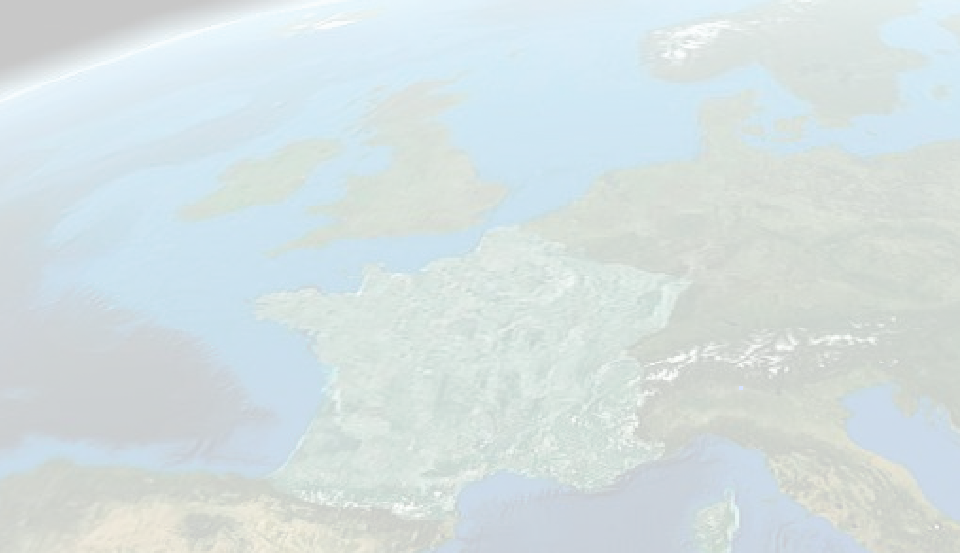
\includegraphics[width=12.5cm]{fondClair.png} };
		\draw (0,5) node[right] { 
\includegraphics[height=1.5cm]{LOGO_IGN.png} };
		\draw (1.5,4.95) node[right] { 
\includegraphics[width=3cm]{fondD.jpg} };
		\end{tikzpicture}   
	}
	\begin{frame}[plain,c]
		\vspace{3cm}
		
\begin{tikzpicture}
		\draw (0,0)node{};
		\draw (4.5,1) node[color =IGNGris, inner sep=0.5em, minimum size=0.5em, text centered,font=\LARGE] { Thanks for your attention, }; 
		\draw (4.5,0) node[color =IGNGris, inner sep=0.5em, minimum size=0.5em, text centered,font=\LARGE] { I am ready for your questions! }; 
		\draw (4.5,-2) node[color =IGNVert, inner sep=0.5em, minimum size=0.5em, text centered,font=\LARGE] { oussama.ennafii@ign.fr }; 
		\end{tikzpicture}
	\end{frame}
	
	
\end{document}
